\documentclass[10pt, a5paper]{article}
\usepackage{pdfpages}
\usepackage{parallel}
\usepackage[T2A]{fontenc}
\usepackage{ucs}
\usepackage[utf8x]{inputenc}
\usepackage[polish,english,russian]{babel}
\usepackage{hyperref}
\usepackage{rotating}
\usepackage[inner=2cm,top=1.8cm,outer=2cm,bottom=2.3cm,nohead]{geometry}
\usepackage{listings}
\usepackage{graphicx}
\usepackage{wrapfig}
\usepackage{longtable}
\usepackage{indentfirst}
\usepackage{array}
\newcolumntype{P}[1]{>{\raggedright\arraybackslash}p{#1}}
\frenchspacing
\usepackage{fixltx2e} %text sub- and superscripts
\usepackage{icomma} % коскі ў матэматычным рэжыме
\PreloadUnicodePage{4}

\newcommand{\longpage}{\enlargethispage{\baselineskip}}
\newcommand{\shortpage}{\enlargethispage{-\baselineskip}}

\def\switchlang#1{\expandafter\csname switchlang#1\endcsname}
\def\switchlangbe{
\let\saverefname=\refname%
\def\refname{Літаратура}%
\def\figurename{Іл.}%
}
\def\switchlangen{
\let\saverefname=\refname%
\def\refname{References}%
\def\figurename{Fig.}%
}
\def\switchlangru{
\let\saverefname=\refname%
\let\savefigurename=\figurename%
\def\refname{Литература}%
\def\figurename{Рис.}%
}

\hyphenation{admi-ni-stra-tive}
\hyphenation{ex-pe-ri-ence}
\hyphenation{fle-xi-bi-li-ty}
\hyphenation{Py-thon}
\hyphenation{ma-the-ma-ti-cal}
\hyphenation{re-ported}
\hyphenation{imp-le-menta-tions}
\hyphenation{pro-vides}
\hyphenation{en-gi-neering}
\hyphenation{com-pa-ti-bi-li-ty}
\hyphenation{im-pos-sible}
\hyphenation{desk-top}
\hyphenation{elec-tro-nic}
\hyphenation{com-pa-ny}
\hyphenation{de-ve-lop-ment}
\hyphenation{de-ve-loping}
\hyphenation{de-ve-lop}
\hyphenation{da-ta-ba-se}
\hyphenation{plat-forms}
\hyphenation{or-ga-ni-za-tion}
\hyphenation{pro-gramming}
\hyphenation{in-stru-ments}
\hyphenation{Li-nux}
\hyphenation{sour-ce}
\hyphenation{en-vi-ron-ment}
\hyphenation{Te-le-pathy}
\hyphenation{Li-nux-ov-ka}
\hyphenation{Open-BSD}
\hyphenation{Free-BSD}
\hyphenation{men-ti-on-ed}
\hyphenation{app-li-ca-tion}

\def\progref!#1!{\texttt{#1}}
\renewcommand{\arraystretch}{2} %Іначай формулы ў матрыцы зліпаюцца з лініямі
\usepackage{array}

\def\interview #1 (#2), #3, #4, #5\par{

\section[#1, #3, #4]{#1 -- #3, #4}
\def\qname{LVEE}
\def\aname{#1}
\def\q ##1\par{{\noindent \bf \qname: ##1 }\par}
\def\a{{\noindent \bf \aname: } \def\qname{L}\def\aname{#2}}
}

\def\interview* #1 (#2), #3, #4, #5\par{

\section*{#1\\{\small\rm #3, #4. #5}}

\def\qname{LVEE}
\def\aname{#1}
\def\q ##1\par{{\noindent \bf \qname: ##1 }\par}
\def\a{{\noindent \bf \aname: } \def\qname{L}\def\aname{#2}}
}

\begin{document}
\title{Кластеризация систем хранения данных с помощью NFS\footnote{\url{inimicus@tut.by}, \url{https://lvee.org/en/abstracts/288}}}
\author{Влад Шарпио, Minsk, Belarus}
\maketitle
\begin{abstract}
A data storage clasterization specifics based on Parallel NFS (pNFS) is reviewed. The pNFS protocol details and architecture-related specifics are covered as well as its current state.
\end{abstract}
\section*{Кластеризация СХД}

Долгое время функция создания кластеров систем хранения данных относилось только к закрытым блочным системам. Популярность дешевых NAS  и потребность в повышенной отказоустойчивости породило цклую плеяду кластерных объектных хранилищ со сложной системой управления и еще более сложными механизмами расчета производительности. В январе  2010 было обубликована спецификация протокола NFS v4.1 RFC 5661 которая позволят использовать несколько NAS  как единое дисковое пространство.

NFS в классическом понимании состоит из серверного и клиентской частей, а тпкаже протоколов взаимодействия между ними. При работе с использованием NFS сервер скрывает реальную  структуру дисковой и файловой системы, предоставляя унифицированную среду, таким образом обеспечивая кроссплатформенное общение.

\section*{Простая конфигурация NFS}

\begin{center}
\begin{figure}[h!]
  \centering
  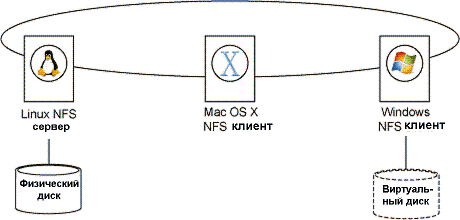
\includegraphics[width=7cm]{16_2018_Sharpio1}
  \caption{Конфигурация NFS v3}
  \label{Sharpio1}
\end{figure}
\end{center} 

Операции по фактическому чтению/записи  данных с/на дисковых или твердотельных накопителей осуществляет NFS-сервер. Вся работа с данными и метаданными возлагается  на  ресурсы сервера. Такой подход в реализации традиционно приводил к низким показателям производительности по операциям в секунду IOPS в случаях использования объектов большого размера или при случайных операциях  с большим числом объектов. Использование точечных методов в решении таких вопросов (агрегация каналов, использование быстрых файловых систем, потоковая компрессия и дедупликация) хоть и поднимало производительность отдельно взятых NAS, но всё равно  достижение уровня SAN  было практически невозможно.

По крайней мере, так было раньше.

Версия NFS 4.1 включает в себя расширение инструкций в области паралелизации работы~--- Parallel NFS (pNFS), что даёт возможность избавиться от недостатков  NFS-хранилища и обеспечить механизм повышения скорости передачи данных (за счёт обеспечения распараллеливания операций ввода/вывода).

При работе с pNFS клиенты, как и раньше, имеют доступ к файловой системе сервера, однако рабочие потоки обработки метаданных и  данных разделены. Сервер метаданных pNFS обеспечивает выполнение фазы инициализации соединения, после чего обемен данным осуществляется между клиентом и сервером NFS. Конфигурация pNFS показана на рисунке~\ref{Sharpio2}.

\begin{center}
\begin{figure}[h!]
  \centering
  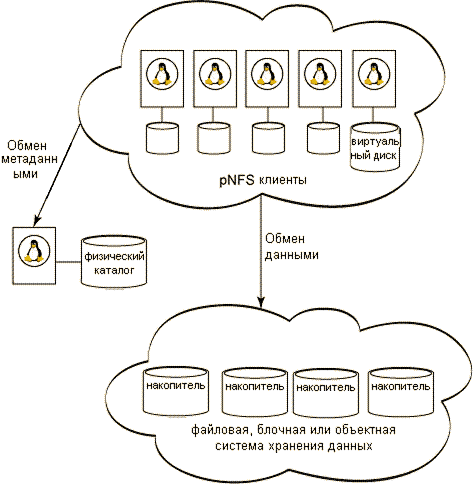
\includegraphics[width=7cm]{16_2018_Sharpio2}
  \caption{Концепция организации pNFS}
  \label{Sharpio2}
\end{figure}
\end{center} 

Задачами  сервера метаданных  является  экспорт файловой системы, хранение и поддержание каноничных метаданных. Клиент новой версии обеспечивает монтирование конечной файловой системы на основании данных pNFS сервера и обеспечивает непосредственное взаимодействие в работе с данными с NFS серверами.

Сервер pNFS не участвует в транзакциях по передаче данных, что повышает производительность.

Такой подход в работе pNFS сохраняет все удобства и преимущества NFS, добавляя к ним производительность и масштабируемость.

\section*{pNFS в деталях}

Протокол pNFS передает метаданные о объектах, в рамках единой разметки (layout), между сервером pNFS и клиентским узлом. layout описывает, как объект распределен в системе хранения данных: например, как он поделен между несколькими носителями; также в layout содержатся атрибуты файла (права доступа и т.д.). Все метаданные сохраняются в файлах разметки и хранится на сервере pNFS, а система хранения данных занимается только вводом/выводом информации.

Протокол доступа к системе хранения данных (Storage access protocol) регулирует работу клиента  с системой хранения данных. Каждый протокол доступа к системе хранения данных работает с индивидуальным layout.

Протокол управления (Control protocol) служит для синхронизации между сервером метаданных и сервером данных. Синхронизация — например, реорганизация файлов на носителях— скрыта от клиентов.

\begin{center}
\begin{figure}[h!]
  \centering
  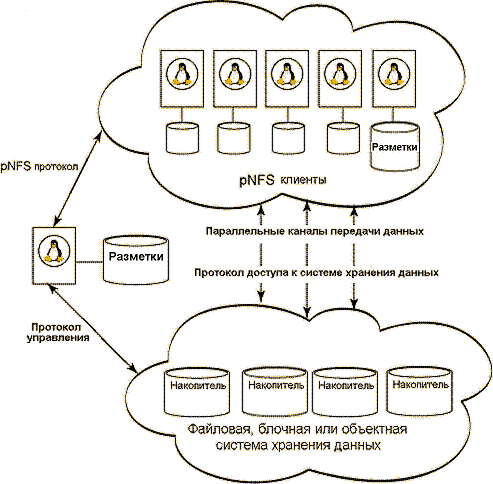
\includegraphics[width=7cm]{16_2018_Sharpio3}
  \caption{Триада протоколов pNFS}
  \label{Sharpio3}
\end{figure}
\end{center} 

Итак, процесс доступа клиента к данным выглядит так:

\begin{enumerate}
  \item Клиент запрашивает разметку файла, с которым предстоит работать.
  \item Клиент получает права доступа путем открытия файла на сервере метаданных.
  \item Авторизовавшись и получив разметку файла, клиент может получать информацию непосредственно с сервера данных. Работа осуществляется в соответствии с протоколом доступа, требуемым для этого типа носителя (подробнее ниже).
  \item Если клиент изменяет файл, клиентская копия разметки изменяется необходимым образом, после чего передается на сервер метаданных.
  \item Когда клиент больше не нуждается в файле, он записывает оставшиеся изменения, передает свою копию разметки обратно на сервер метаданных и закрывает файл.
\end{enumerate}

Более подробно операция чтения (READ) – это серия следующих операций протокола:

\begin{enumerate}
  \item Клиент посылает запрос LOOKUP+OPEN на сервер pNFS. Сервер возвращает дескриптор файла (file handle) и информацию о состоянии файла.
  \item Клиент запрашивает с сервера разметку с помощью команды LAYOUTGET. Сервер возвращает разметку файла.
  \item Клиент посылает запрос READ на устройства хранения, которые инициируют множество параллельных операций READ.
  \item Когда клиент заканчивает чтение, он посылает команду\\ LAYOUTRETURN.
  \item Если клиентская копия разметки становится неактуальной (из-за изменения серверной разметки каким-либо другим, выполняющимся параллельно действием), сервер посылает команду CB\_LAYOUTRECALL, сообщая, что разметка уже не действительна и ее надо обновить.
\end{enumerate}

Операция Write выглядит так же, за исключением того, что клиент шлет команду LAYOUTCOMMIT перед командой\\ LAYOUTRETURN, чтобы «опубликовать» свои изменения файла на сервере pNFS.

Разметки могут кэшироваться на каждом клиенте, что еще больше повышает скорость работы. Также клиент может при желании удалять свою копию разметки полученной с сервера, если она больше не используется. Также сервер позволяет ограничивать в разметке размер записываемых данных, чтобы, например, не использовать дисковые квоты или уменьшить издержки на выделение ресурсов.

Для того чтобы данные в кэше оставались актуальными, сервер метаданных отзывает устаревшие разметки. Все затронутые отзывом клиенты должны приостановить работу с данными и, либо обновить свою версию разметки, либо продолжить работу через обыкновенную NFS. Сервер обязательно делает отзыв разметки перед началом административной работы с файлом (например, миграции или изменения распределения файла по системам хранения).

Независимо от типа разметки pNFS использует для обращения к серверам общую схему. Вместо имени хоста или тома накопителя обращение к серверам происходит по уникальным идентификаторам. Этому идентификатору ставится в соответствие зависящая от конкретного протокола доступа ссылка на сервер.

Какой из этих методов хранения лучше? Ответ индивидуален и зависит от размера бюджета, масштаба системы, требуемой скорости, простоты работы и других факторов.

\section*{Текущее состояние pNFS}

Нативная поддержка протокола на уровне ядра доступна с версий
2.6.37, поддержка всего функционала полностью реализована в ветке 3.1.

Мейнтейнером развития является коммерческая организация \\Panasas,  активная часть сообщества~--- 118 аккаунтов.

Основная ветка развития протокола 4.1 завершена в 2010 году.
С 2014 и по настоящее время идёт стандартизация (формально завершена в 2016) и развитие  ветки 4.2.

\begin{thebibliography}{20}
  \bibitem{Sharpio-1} \url{https://www.snia.org/sites/default/files/NFS\_4.2\_Final.pdf}
  \bibitem{Sharpio-2} \url{http://linux-nfs.org}
  \bibitem{Sharpio-3} \url{https://www.ibm.com/developerworks/ru/library/l-pnfs}
  \bibitem{Sharpio-4} \url{https://tools.ietf.org/html/rfc7862}
  \bibitem{Sharpio-5} \url{https://tools.ietf.org/html/rfc5661}
\end{thebibliography}

\end{document}
